\chapter{Extending our work to Deep CCA and Self-Supervised Learning: A Powerful Approach to Multiview Nonlinear Association Learning}
\label{Deep}

\section{Introduction}

\section{Data}

\subsection{Split MNIST}
The Split MNIST dataset \cite{wang2015stochastic} is a standard benchmark for DCCA. It consists of 60,000 images of handwritten digits from the MNIST dataset \cite{lecun1998gradient}. Each image is 28\times28 pixels with 1 channel but we split the image into two halves, each of size 28\times14 pixels. We use the standard train/test split.

\subsection{XRMB}
The X-Ray Microbeam (XRMB) dataset \cite{westbury1994x} is a multimodal dataset of speech recordings from 139 speakers with acoustic and articulatory features. The acoustic features are 39-dimensional Mel-frequency cepstral coefficients (MFCCs) extracted from the speech recordings. The articulatory features are 12-dimensional vectors of the vertical positions of the tongue, lips, and jaw. The dataset contains 1,429,236 frames of data, with 10,302 frames per speaker. We use the standard train/test split.

\subsection{CIFAR-10 and CIFAR-100}
The CIFAR-10 and CIFAR-100 datasets contain 60,000 images each, with 10 and 100 classes respectively. Each image is 32\times32 pixels with 3 channels. We use the standard train/test split.


\section{Methods}

\subsection{DCCA-EY and DCCA-SVD: Extension to Deep CCA}\label{sec:deep-cca}
The GEP-EY and CCA-SVD formulations also lead naturally to new formulations of Deep CCA which solve a more flexible CCA problem but unlike prior work can be optimized efficiently in the stochastic setting. We will refer to these as DCCA-EY and DCCA-SVD.

%L; just moved this up
We derive the DCCA-EY formulation by applying the GEP formulation of CCA (\ref{eq:cca-GEV}) to our DCCA definition. The analogous derivation for DCCA-SVD is left to supplement \ref{supp:algorithm-details}. 

Population DCCA \cite{andrew2013deep} can be defined analogously to population CCA (see section \ref{sec:CCA Definition}):
% Following the definition of CCA in section \ref{sec:CCA Definition}, the population formulation of DCCA \cite{andrew2013deep}, can be defined as follows: 
given input random vectors $X \in \R^{D_x}, Y \in \R^{D_y}$, find neural networks $f,g$ maximising:
\begin{align}\label{eq:DCCA-Andrew}
    \max_{f,g}  \norm{\CCA_K\left(f(X),g(Y)\right)}_2
\end{align}

The GEP formulation becomes:
\begin{equation*}
    A_{fg} = \begin{pmatrix} 0 &\Cov(f(X),g(Y)) \\ \Cov(g(Y),f(X)) & 0 \end{pmatrix}, \qquad
	B_{fg} = \begin{pmatrix}\Var(f(X)) & 0 \\ 0 & \Var(g(Y)) \end{pmatrix}.
\end{equation*}

Proposition \ref{prop:EY-charac} then allows us to rewrite our objective (\ref{eq:DCCA-Andrew}) as:
\begin{align*}
    \norm{\CCA_k\left(f(X),g(Y)\right)}^2 
    = \sum_{j=1}^k \rho_j^2 
    = \max_{W \in \R^{d \times k}} \tr \left( 2\, W^T A_{fg} W - \left(W^T B_{fg} W\right) \left(W^T B_{fg} W\right) \right).
\end{align*}
Therefore DCCA is equivalent to maximising the right hand side with respect to $f,g$ and $W$. To simplify the objective we follow \cite{wang2015stochastic} and reparametrize to consider the `augmented' neural networks $\bar{f} = U^{\top} f, \bar{g} = V^{\top} g$, where $U\in \R^{d_x \times k}, V\in \R^{d_y \times k}$ are such that $W^{\top} = (U^{\top}, V^{\top})$. This gives our final DCCA objective:

\begin{align}\label{eq:DCCA-EY}
    \mathcal{U}^\text{DCCA-EY}(\bar{f},\bar{g}) = \tr(2 \, A_{\bar{f}\bar{g}} - B_{\bar{f}\bar{g}} B_{\bar{f}\bar{g}})
\end{align}

where we need to define:
\begin{align*}
    A_{\bar{f}\bar{g}}
    &= W^T A_{fg} W 
    = \Cov(\bar{f}(X),\bar{g}(Y)) + \Cov(\bar{g}(Y),\bar{f}(X)) \\
    B_{\bar{f}\bar{g}} 
    &= W^T B_{fg} W 
    = \Cov(\bar{f}(X)) + \Cov(\bar{g}(Y))
\end{align*}


By plugging in sample covariances on a minibatch, we can obtain unbiased estimates of $\mathcal{U}^\text{DCCA-EY}(\bar{f},\bar{g})$.

Therefore, we can apply some variant of SGD to optimize equation \ref{eq:DCCA-EY}.

Note that, as in the earlier DCCA work, though we derived the algorithm by considering $f,g$ with output dimensions $d_x,d_y$, we ultimately end up with networks $\bar{f},\bar{g}$ with the same output dimension $k$; we can view these as giving highly correlated $k$-dimensional embeddings of our data.

\subsection{SSL-EY and SSL-SVD: Application to Self-Supervised Learning}

Finding highly correlated embeddings is a natural objective for SSL.
To apply the previous ideas to joint embedding methods, we simply apply (\ref{eq:DCCA-EY}) in the Siamese pair setting where $\bar{f}=\bar{g}$ are the same map from input data to embeddings (composition of encoder and projector).

We therefore obtain the objective:
\begin{align}\label{eq:SSL-EY}
    \mathcal{U}^\text{SSL-EY}(\bar{f}) =\tr( 2 \, A_{\bar{f}} - B_{\bar{f}} B_{\bar{f}})
\end{align}
where:
\begin{align*}
    A_{\bar{f}}
    &= \Cov(\bar{f}(X),\bar{f}(X')) + \Cov(\bar{f}(X'),\bar{f}(X)) \\
    B_{\bar{f}} 
    &= \Var(\bar{f}(X)) + \Var(\bar{f}(X')).
\end{align*}

Once again, we define SSL-SVD by analogy in supplement \ref{supp:algorithm-details}. We will see in section \ref{Experiments} that SSL-SVD and SSL-EY perform similarly in experiments but we show in supplement \ref{supp:previous work} that the SSL-SVD formulation looks closer to existing SSL methods.

\textbf{Implementation Details:} Typical architectures for the encoder and the projector vary depending on the domain and the dataset \cite{balestriero2023cookbook}. For example, for image classification tasks on CIFAR-10 or ImageNet, a common choice for the encoder is a ResNet, while for the projector a linear layer or a two-layer MLP is often used. Common augmentations for images are cropping, flipping, rotating, color jittering, etc. In this work, we adopt standard architectures and augmentations from the literature.


\section{Experiments and Results}

%%%%%%%%%%%%%%%%%%%%%%%%%%%%%%%%%%%%%%%%%%%%%%%%%%%%%%%%%%%%%%%%%%%%%%%%%%%%%%%%%%%%%%
%DCCA Benchmarking
%%%%%%%%%%%%%%%%%%%%%%%%%%%%%%%%%%%%%%%%%%%%%%%%%%%%%%%%%%%%%%%%%%%%%%%%%%%%%%%%%%%%%%
\subsection{Application of DCCA-EY and DCCA-SVD to to Deep multiview learning on toy data}

We now turn to compare our proposed DCCA-EY and DCCA-SVD methods with existing methods for deep canonical correlation analysis (DCCA). We replicate an experiment from \cite{wang2015stochastic} using the left and right halves of MNIST \cite{lecun1998gradient} digits ($n$=60,000) and X-Ray Microbeam (XRMB, $n$=1,429,236) data \cite{westbury1994x}. XRMB is a multimodal dataset of speech recordings from 139 speakers with acoustic and articulatory features. We use minibatch sizes of 100 for 20 epochs, the architectures described in \cite{wang2015stochastic}, and an output dimensionality of 50.  We use the total correlation captured (TCC) of the learnt subspace on the validation set as a metric (defined in supplement \ref{supp:experimental details}).

\begin{figure}
     \centering
     \begin{subfigure}[b]{0.49\textwidth}
         \centering
         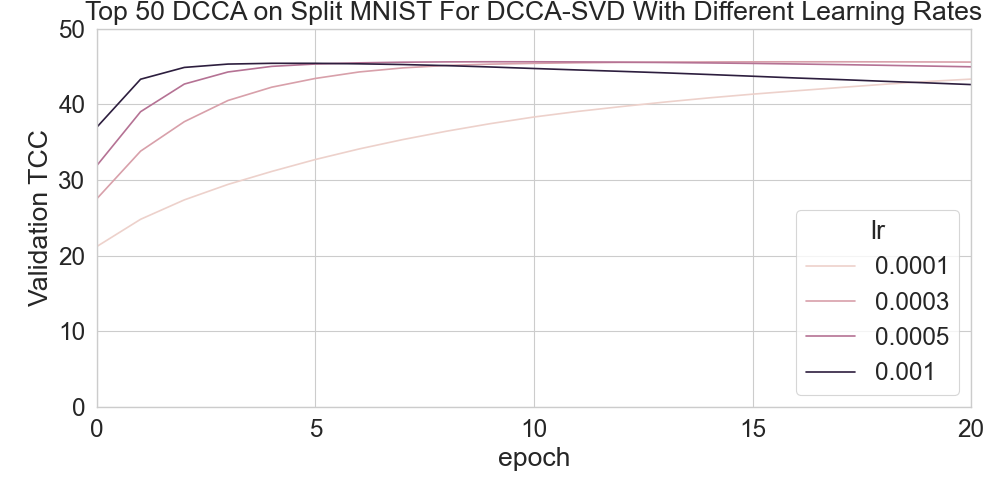
\includegraphics[width=\textwidth]{figures/DCCA/dcca_lr_experiment.png}
         \caption{}
         \label{fig:lrexp}
     \end{subfigure}
     \hfill
     \begin{subfigure}[b]{0.49\textwidth}
         \centering
         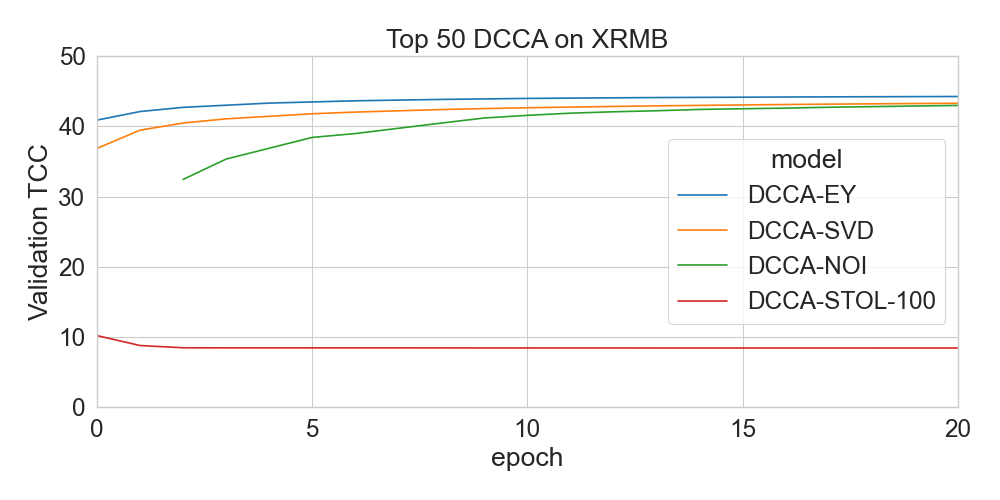
\includegraphics[width=\textwidth]{figures/DCCA/dcca_XRMB.png}
         \caption{}
                 \label{fig:xrmb}
     \end{subfigure}
        \caption{ (a) Validation TCC for different learning rates on Split MNIST data (b) Validation TCC for different methods on XRMB data}

\end{figure}

On the split MNIST data, we show in figure \ref{fig:lrexp} the substantial effect of changing the learning rate on the convergence of the TCC objective. This demonstrates the important of spending computational resource on optimizing the learning rate. An important benefit of our approach is that because the only hyperparameter is learning rate, we can spend all of our computational budget on this critical area. In figure \ref{fig:xrmb}, we show that our proposed methods exhibit extremely fast convergence compared to prior work. Furthermore, both proposed methods find higher validation correlations than DCCA-STOL, showing that they are much more effective ways of estimating the full batch DCCA objective. Note that, the decrease in validation correlation in later epochs is due to overfitting which should be addressed in practical settings by using early stopping as is standard in deep learning.

%%%%%%%%%%%%%%%%%%%%%%%%%%%%%%%%%%%%%%%%%%%%%%%%%%%%%%%%%%%%%%%%%%%%%%%%%%%%%%%%%%%%%%
%SSL
%%%%%%%%%%%%%%%%%%%%%%%%%%%%%%%%%%%%%%%%%%%%%%%%%%%%%%%%%%%%%%%%%%%%%%%%%%%%%%%%%%%%%%
\subsection{Application of SSL-EY and SSL-SVD to Self-Supervised Learning}

In this section, we test our SSL objectives on the CIFAR-10 and CIFAR-100 datasets, which both have 60,000 images and 10 and 100 classes respectively. We compare our methods, SSL-EY and SSL-SVD, with two state-of-the-art methods, Barlow Twins and VICReg. We report k-Nearest Neighbor accuracy on the representations of the validation data in a zero-shot setup.

Firstly, we consider a standard experiment from the literature.
We use the sololearn package \cite{da2022solo}, which includes optimised hyperparameters (and augmentations) for VICReg and Barlow Twins on this specific task.
Each method uses a ResNet-18 encoder, a two-layer projector network with 2048 units in each layer, and is trained for 1,000 epochs with a minibatch size of 256.
For SSL-EY and SSL-SVD, we use the same hyperparameters as Barlow Twins.  
Table \ref{tab:selfsup} shows that our methods are competitive with Barlow Twins and VICReg in this setup.
This is remarkable because their tuning parameters had been heavily optimised, and our method required no tuning at all!

We then performed ablation studies to understand the importance of the (many) hyperparameters in these joint embedding models. In general we found that VICReg was much more sensitive to these hyperparameters than Barlow Twins but that our method was significantly more stable than either of them, see supplement \ref{supp:ablation}.
Table \ref{tab:selfsupsmaller} shows a particularly striking example of this. 
We repeat the previous experiment with all hyperparameters the same apart from the projector: we take a smaller projector with only 256 units in each layer. 
Comparing Tables \ref{tab:selfsup} and \ref{tab:selfsupsmaller} shows that VICReg and Barlow Twins have a large performance drop with the smaller projector on the non-trivial classification problems; our methods are much less affected, and now significantly outperform VICReg and Barlow Twins.
 

\begin{table}[h] 
\centering 
\begin{tabular}{lcccc} 
\hline 
Method & CIFAR-10 Top-1 & CIFAR-10 Top-5 & CIFAR-100 Top-1 & CIFAR-100 Top-5 \\ 
\hline 
Barlow Twins & \textbf{92.1} & 99.73 & \textbf{71.38} & \textbf{92.32}\\
VICReg & 91.68	&99.66 & 68.56&	90.76 \\
\textbf{SSL-EY} & 91.43& \textbf{99.75}& 67.52& 90.17\\
\textbf{SSL-SVD} & 90.57 & 99.71 & 65.93 & 89.31 \\
\hline 
\end{tabular} \caption{SSL methods on CIFAR-10 and CIFAR-100 using 2048 unit projectors.} \label{tab:selfsup}
\centering 
\begin{tabular}{lcccc} 
\hline 
Method & CIFAR-10 Top-1 & CIFAR-10 Top-5 & CIFAR-100 Top-1 & CIFAR-100 Top-5 \\ 
\hline 
Barlow Twins & 88.35 & \textbf{99.71} & 59.94 & 85.99 \\
VICReg & 88.74 & 99.68 & 57.03& 84.45 \\
\textbf{SSL-EY} & 89.49 & 99.54 & \textbf{65.62}& \textbf{89.00}\\
\textbf{SSL-SVD} & \textbf{90.34} & 99.67 & 64.54 & 88.66 \\
\hline 
\end{tabular} \caption{SSL methods on CIFAR-10 and CIFAR-100 using 256 unit projectors.} \label{tab:selfsupsmaller} \end{table}

\section{Discussion and Conclusion}





